\documentclass[10pt,a4paper]{article}

% for greek
\usepackage{xltxtra} 
\usepackage{xgreek} 
\usepackage{fontspec} 
\setromanfont{Roboto}
\usepackage[utf8]{inputenc}

% for references link
	%link into artivle to go to refernces
	\usepackage{hyperref} 
	%link to go to urls
	\usepackage{url}

% bibliography
%\usepackage[backend=bibtex]{biblatex}   

% for code
\usepackage{listings}
\usepackage{xcolor}

% figures
\usepackage{graphicx}
\usepackage{float}

% bulleted list
\usepackage{blindtext}
\usepackage{enumitem}

\lstdefinestyle{customc}{
  belowcaptionskip=1\baselineskip,
  breaklines=true,
  xleftmargin=\parindent,
  language=C++,
  showstringspaces=false,
  basicstyle=\footnotesize\ttfamily,
  keywordstyle=\bfseries\color{green!40!black},
  commentstyle=\itshape\color{purple!40!black},
  identifierstyle=\color{blue},
  stringstyle=\color{orange},
}

\lstset{escapechar=@,style=customc}
 
\title{Κατασκευή REST API και Web Εφαρμογής}
\author{Πασχαλίδης Παύλος\\ΤΕΙ ΘΕΣΣΑΛΙΑΣ\\msf7415012@teilar.gr}
\date{}

\begin{document}

	\pagenumbering{gobble}
	
	\maketitle
	\newpage	
			
	\begin{abstract}
	Το αντικείμενο της παρούσας αναφοράς είναι η επεξήγηση της διαδικασίας για την δημιουργία μιας αλληλεπιδραστικής web εφαρμογής που τροφοδοτείται με δεδομένα μέσω ενός web API τύπου REST στα πλαίσια του μαθήματος Προηγμένες Web Εφαρμογές του μεταπτυχιακού προγράμματος σπουδών με τίτλο ''Μηχανική Λογισμικού για Διαδικτυακές και Φορητές Εφαρμογές'' του τμήματος Μηχανικών Πληροφορικής του ΤΕΙ Θεσσαλίας.
	\end{abstract}

	\pagenumbering{arabic}
	
	\tableofcontents	
	\newpage
	
	\begin{appendix}
	  \listoffigures
%	  \listoftables
	\end{appendix}

			
%	\input{intro}
	\section{Εργαλεία Και Τεχνικές}
\subsection{Πλαίσιο Λογισμικού - PHP}
Για την υλοποίηση του REST API χρησιμοποιήθηκε το framework\footnotemark\footnotetext{Software framework, a reusable set of libraries or classes for a software system} \textbf{Lumen-Laravel} \cite{lumen-laravel} που ενδείκνυται για το σκοπό αυτό. Ωστόσο τα προαπαιτούμενα για την χρήση του framework είναι:  

\begin{itemize}
\item PHP >= 5.6.4
\item OpenSSL PHP Extension
\item PDO PHP Extension
\item Mbstring PHP Extension
\end{itemize}

τα οποία ήταν διαφορετικά στο τοπικό υπολογιστή μου (PHP 5.61) και για το λόγο αυτό χρησιμοποιήθηκε το εικονικό περιβάλλον \textbf{Laravel Homstead} \cite{laravel-homestead} με τη χρήση VirtualBox\footnotemark\footnotetext{Oracle VM VirtualBox, supports the creation and management of virtual machines} και Vagrant\footnotemark\footnotetext{Open-source software for building and maintaining porable virtual devepment enviroments}.

\subsection{Περιβάλλον Ανάπτυξης}

Το \textbf{Laravel Homstead}\cite{laravel-homestead} είναι ένα επίσημο πακέτο Vagrant box που παρέχει ένα περιβάλλον ανάπτυξης χωρίς να απαιτείται η εγκατάσταση PHP, Web Server και άλλα προγράμματα λογισμικού στο τοπικό υπολογιστή.

Περιλαμβάνει τα εξής λογισμικά:

\begin{itemize}
\item Ubuntu 16.04
\item Git
\item PHP 7.1
\item Nginx
\item MySQL
\item MariaDB
\item Sqlite3
\item Postgres
\item Composer
\item Node (With Yarn, PM2, Bower, Grunt, and Gulp)
\item Redis
\item Memcached
\item Beanstalkd
\end{itemize}

\subsection{Σύστημα Ελέγχου Εκδόσεων}

Για την διαχείριση των εκδόσεων του Rest API και του Web Application χρησιμοποιήθηκε το git\footnotemark\footnotetext{Free sofware, used for software development and other version control tasks} και ένα private repository απο το git-hub\footnotemark\footnotetext{Web-based gii repository hosting service}

\begin{figure}[H]
  \caption{Εικόνα από το private repository με τα τελευταία commits.}
  \centering
    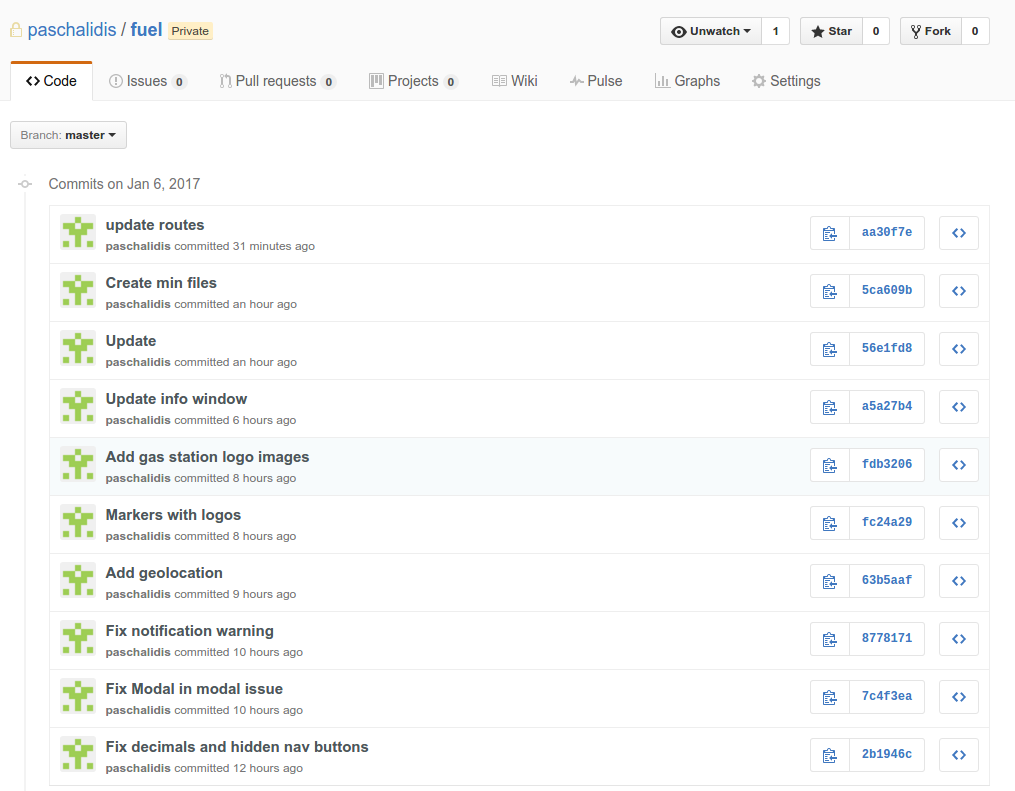
\includegraphics[width=1\textwidth]{img/git.png}
    \label{fig:git}
\end{figure}

\subsection{Βάση Δεδομένων}
Για λόγους ευχρηστίας έγινε πρόσθεση του πεδίου \textbf{id} στους πίνακες \textbf{pricedata} και \textbf{gasstations}, ενώ για τα δικαιώματα των χρηστών (πελάτης, πρατηριούχος) υλοποιήθηκε με το σχεσιακό μοντέλο \textbf{users-and-rights-schema} περισσότερες λεπτομέρειες στο σχεσιακό σχήμα.\ref{fig:db}. Επιπλέον δημιουργήθηκαν τρία views: user-permission, fuel-analytics, pricedata-view.

\begin{figure}[H]
  \caption{Εικόνα από το Σχεσιακό Μοντέλο.}
  \centering
    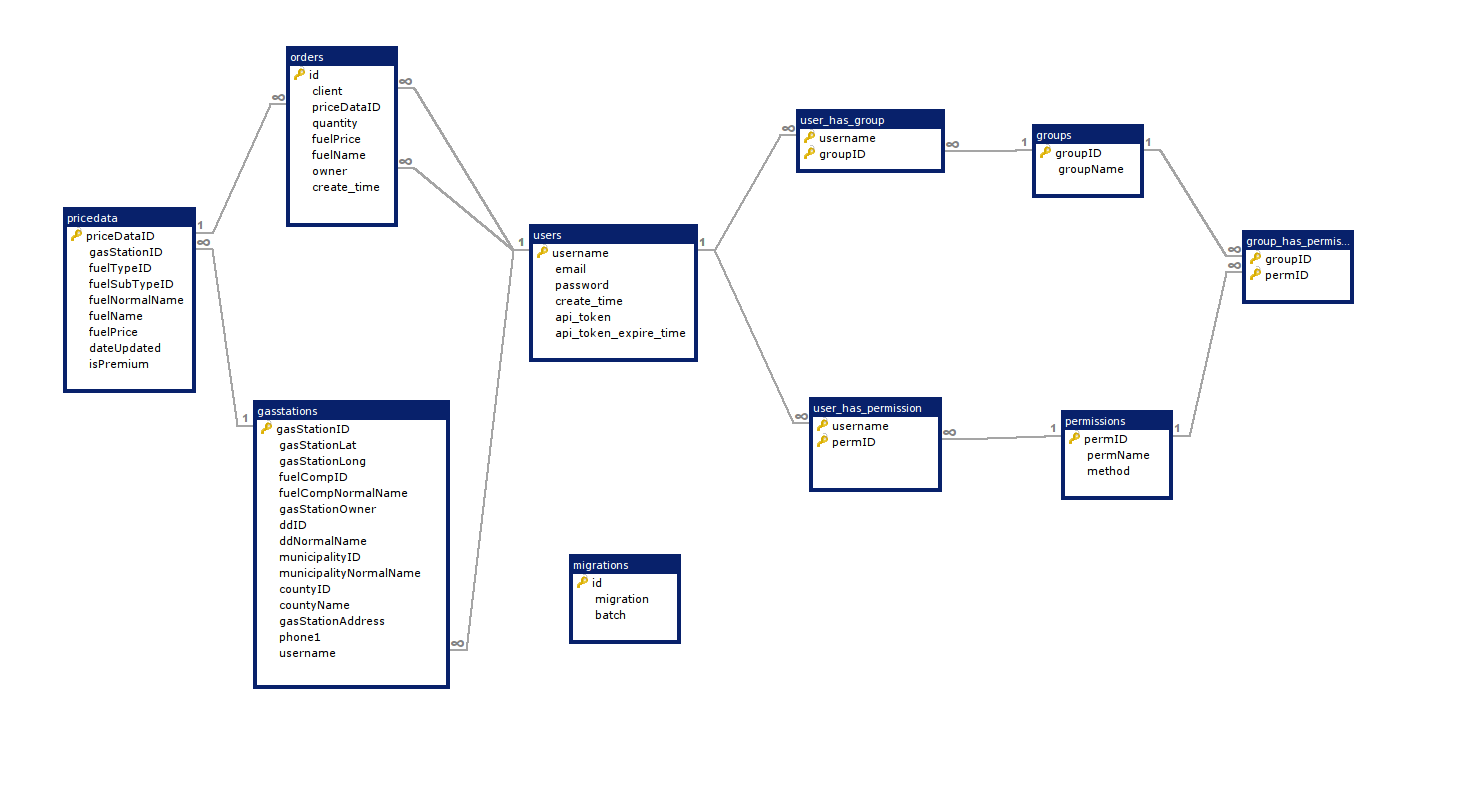
\includegraphics[width=1\textwidth]{img/db-schema.png}
    \label{fig:db}
\end{figure}

\subsection{Καλές Πρακτικές API}
Χρησιμοποιήθηκαν καλές πρακτικές σχεδίασης όπως αυτές παρουσιάστηκαν στις διαλέξεις και για τον έλεγχο και την υλοποίηση των resources η εφαρμογή chrome-postman \cite{chrome-postman}. API URL: \textbf{domain/api/v1/}

\subsubsection{API Resources}
\begin{itemize}
\item GET - gasstations
\item GET - gasstations/count
\item GET - gasstations/id/pricedata
\item GET - pricedata
\item GET - gasstations/analytics
\item POST - login
\item POST - register
\item PUT - pricedata/id
\item POST - orders
\item GET - orders
\end{itemize}

\subsubsection{Fields}
Επιλογή συγκεκριμένων πεδίων με την παράμετρο fields, πχ fields=gasStationID,gasStationLat. \ref{fig:format}

\subsubsection{Where}
Υλοποίηση where statement με το όνομα του πεδίου και την τιμή ή τις τιμές για IN, πχ   gasStationID=1 ή  gasStationID=1,2,3. \ref{fig:format}

\subsubsection{Pagination}
Χρήση pagination με τις εντολές limit και offset και την τιμή του καθενός, πχ limit=10,offset=100. \ref{fig:limit}

\begin{figure}[H]
  \caption{Εικόνα από το API Request Limit και Between.}
  \centering
    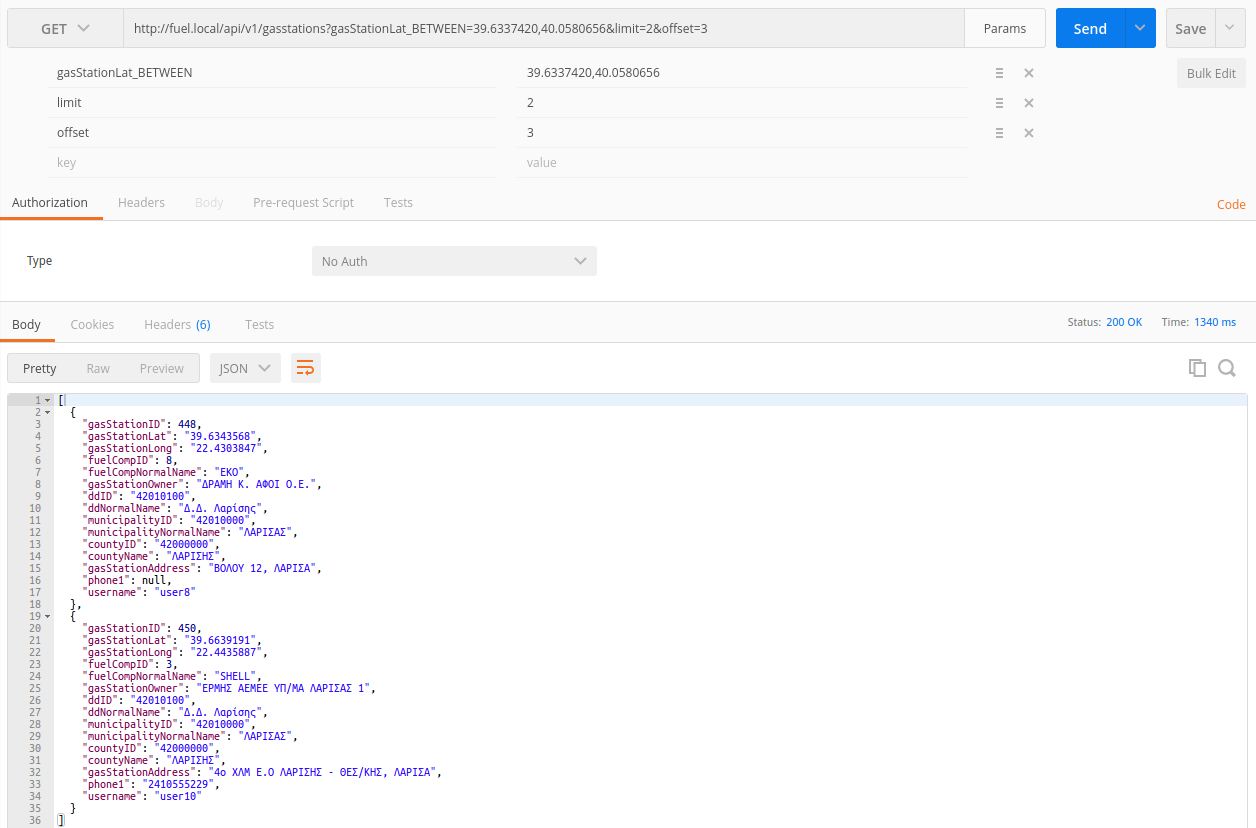
\includegraphics[width=1\textwidth]{img/limit.png}
    \label{fig:limit}
\end{figure}

\subsubsection{Aggregate}
Υλοποίηση συναρτήσεων max, min, avg, count πχ  max=fuelPrice. \ref{fig:aggregate}

\begin{figure}[H]
  \caption{Εικόνα από το API Request με συναρτήσεις και group by.}
  \centering
    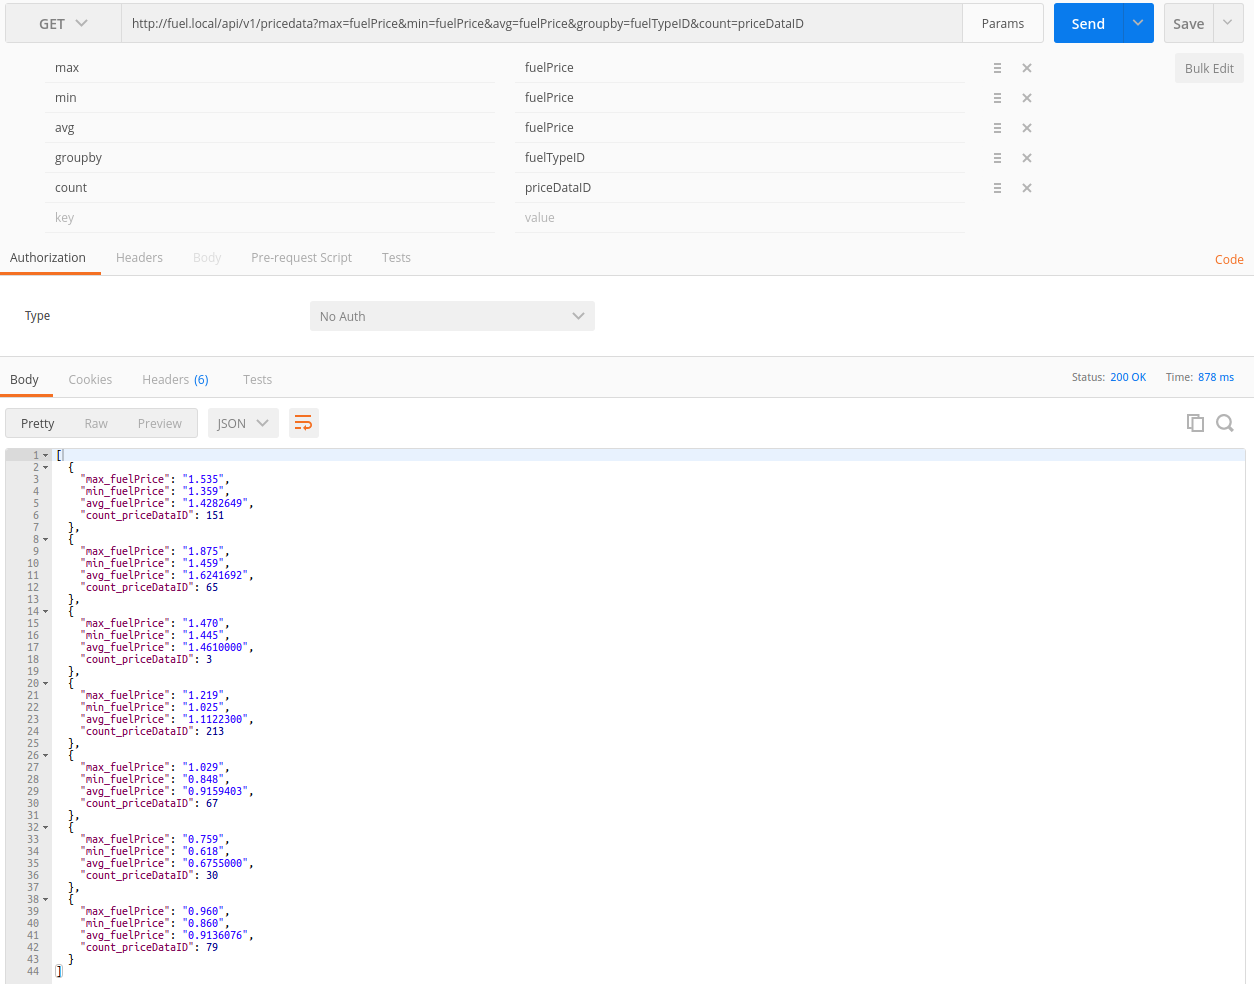
\includegraphics[width=1\textwidth]{img/aggregate.png}
    \label{fig:aggregate}
\end{figure}

\subsubsection{Group By}
Επιλογή για groupby με την παράμετρο groupby, πχ groupby=fuelTypeID. \ref{fig:aggregate}

\subsubsection{Between}
Υλοποίηση του between, πχ gasStationLat\_BETWEEN=39.6337420,40.0580656. \ref{fig:limit}

\subsubsection{Formats}
Επιλογή μορφή δεδομένων με την παράμετρο type=json ή xml. \ref{fig:format}

\begin{figure}[H]
  \caption{Εικόνα από το API Request XML Format.}
  \centering
    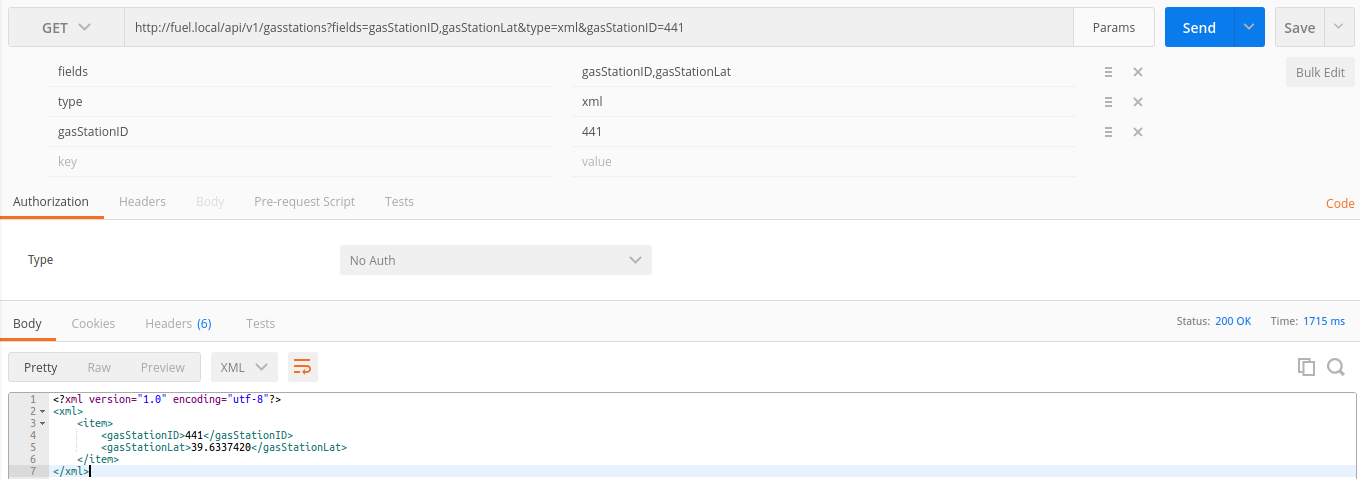
\includegraphics[width=1\textwidth]{img/format.png}
    \label{fig:format}
\end{figure}

\subsubsection{HTTP error}
Με την παράμετρο suppress\_response\_code το API επιστρέφει πάντα http status 200 με μήνυμα λάθους και το response status που θα έπαιρνε. Χωρίς \ref{fig:error} Με \ref{fig:suppress}

\begin{figure}[H]
  \caption{Εικόνα από το API Request με error.}
  \centering
    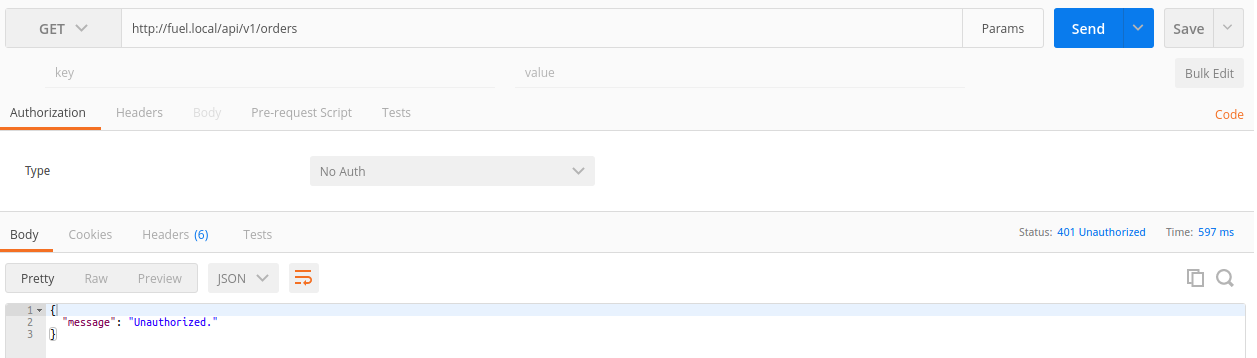
\includegraphics[width=1\textwidth]{img/error.png}
    \label{fig:error}
\end{figure}

\begin{figure}[H]
  \caption{Εικόνα από το API Request με error και suppress response.}
  \centering
    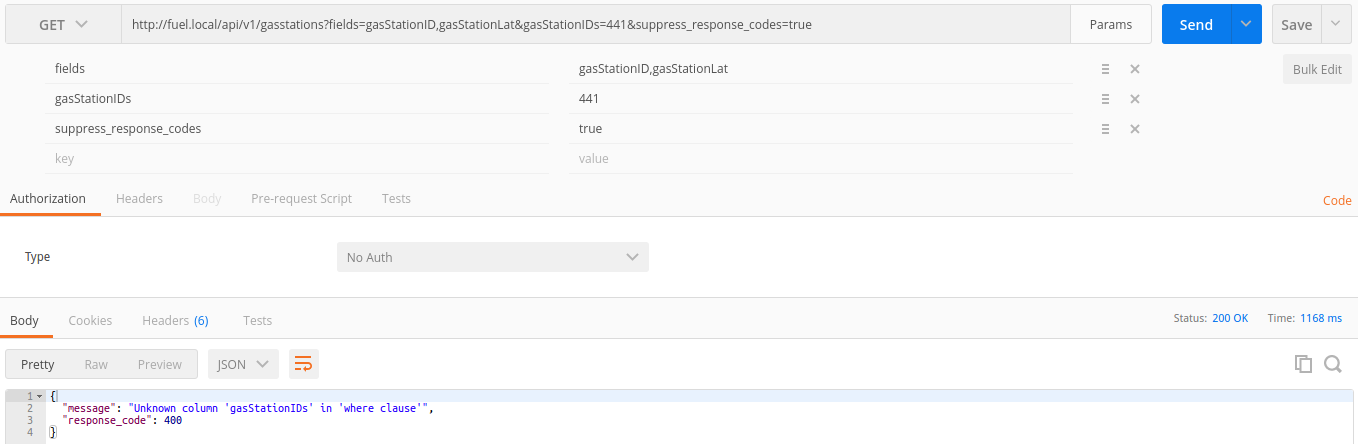
\includegraphics[width=1\textwidth]{img/suppress.png}
    \label{fig:suppress}
\end{figure}

\subsection{Πλαίσιο Λογισμικού - CSS,JS}
Για την υλοποίηση της εφαρμογής Single Page RIA χρησιμοποιήθηκε το framework \textbf{Βootsrap} \cite{bootstrap}
το οποίο παρέχει πολλές λειτουργίες σε HTML, CSS και JS. Για τις ajax κλήσης χρησιμοποιήθηκε η βιβλιοθήκη \textbf{jQuery} \cite{jquery} που είναι εύχρηστη και για τα μηνύματα προς τον χρήστη το plugin \textbf{Notify.js} \cite{notify}.

	\section{Περιπτώσεις Χρήσης}
\subsection{Εγγραφή χρήστη}

\begin{figure}[H]
  \caption{Εικόνα με Εγγραφή χρήστη.}
  \centering
    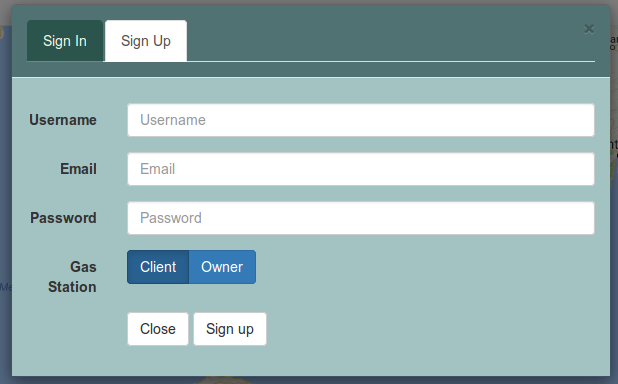
\includegraphics[width=1\textwidth]{img/register.png}
    \label{fig:register}
\end{figure}

\begin{figure}[H]
  \caption{Εικόνα με Εγγραφή χρήστη και λάθος.}
  \centering
    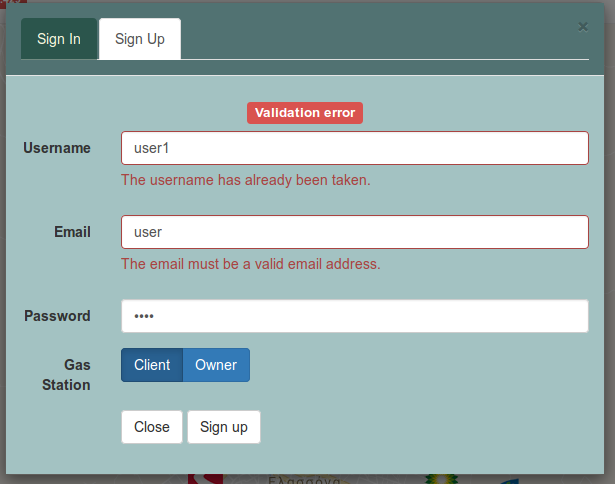
\includegraphics[width=1\textwidth]{img/register-error.png}
    \label{fig:register-error}
\end{figure}

\subsection{LogIn χρήστη}

\begin{figure}[H]
  \caption{Εικόνα με login χρήστη.}
  \centering
    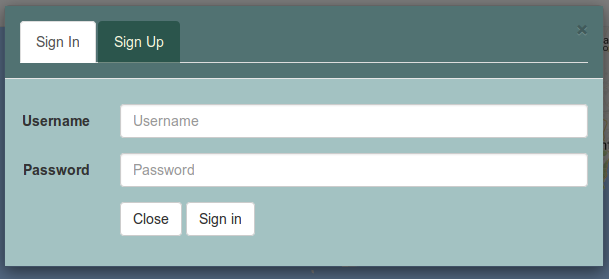
\includegraphics[width=1\textwidth]{img/login.png}
    \label{fig:login}
\end{figure}

\begin{figure}[H]
  \caption{Εικόνα με login χρήστη και λάθος.}
  \centering
    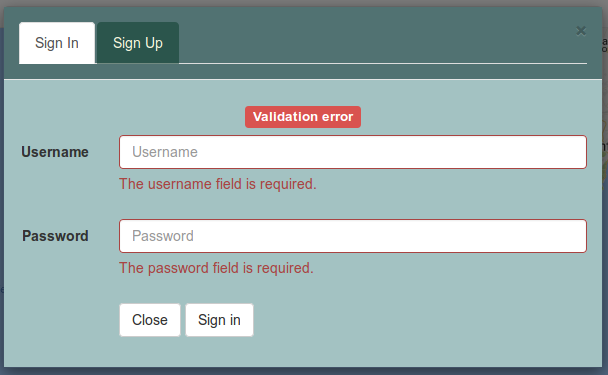
\includegraphics[width=1\textwidth]{img/login-error.png}
    \label{fig:login-error}
\end{figure}

\begin{figure}[H]
  \caption{Εικόνα με login χρήστη success.}
  \centering
    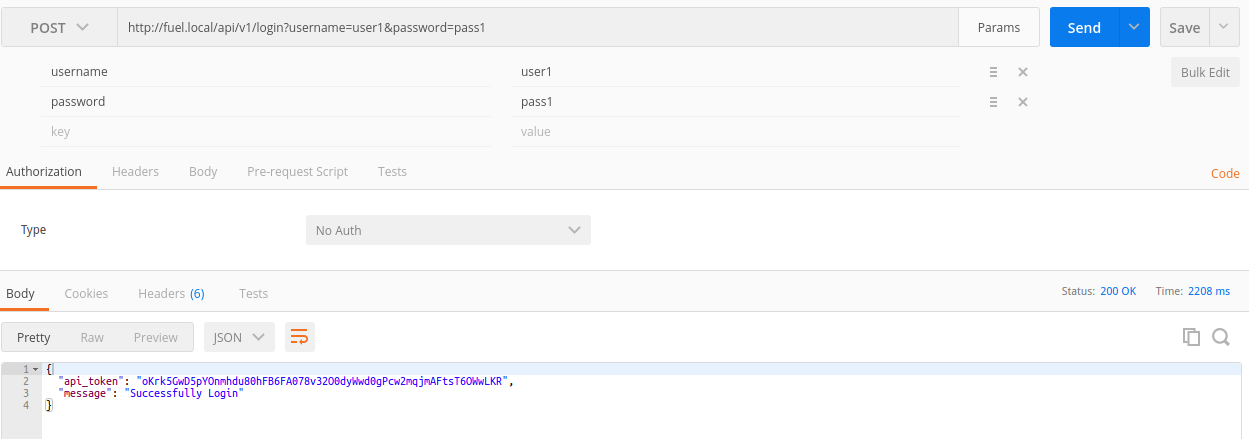
\includegraphics[width=1\textwidth]{img/login-post.png}
    \label{fig:login-post}
\end{figure}

\subsection{Πλήθος πρατηρίων}

\begin{figure}[H]
  \caption{Εικόνα με το Πλήθος πρατηρίων.}
  \centering
    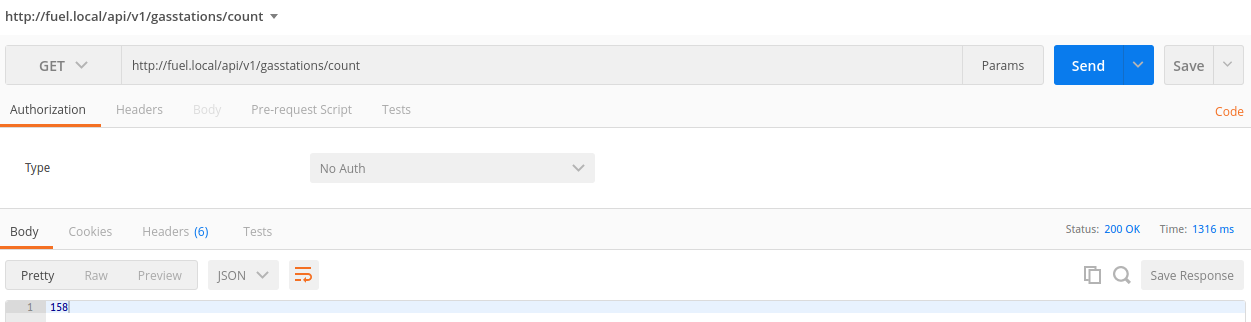
\includegraphics[width=1\textwidth]{img/count.png}
    \label{fig:count}
\end{figure}

\subsection{Λήψη μέγιστης, ελάχιστης και μέσης τιμής}

\begin{figure}[H]
  \caption{Εικόνα μέγιστης, ελάχιστης και μέσης τιμής από την εφαρμογή.}
  \centering
    
\includegraphics[width=1\textwidth]{img/max-min.png}
    \label{fig:max-min}
\end{figure}

\begin{figure}[H]
  \caption{Εικόνα μέγιστης, ελάχιστης και μέσης τιμής από το request.}
  \centering
    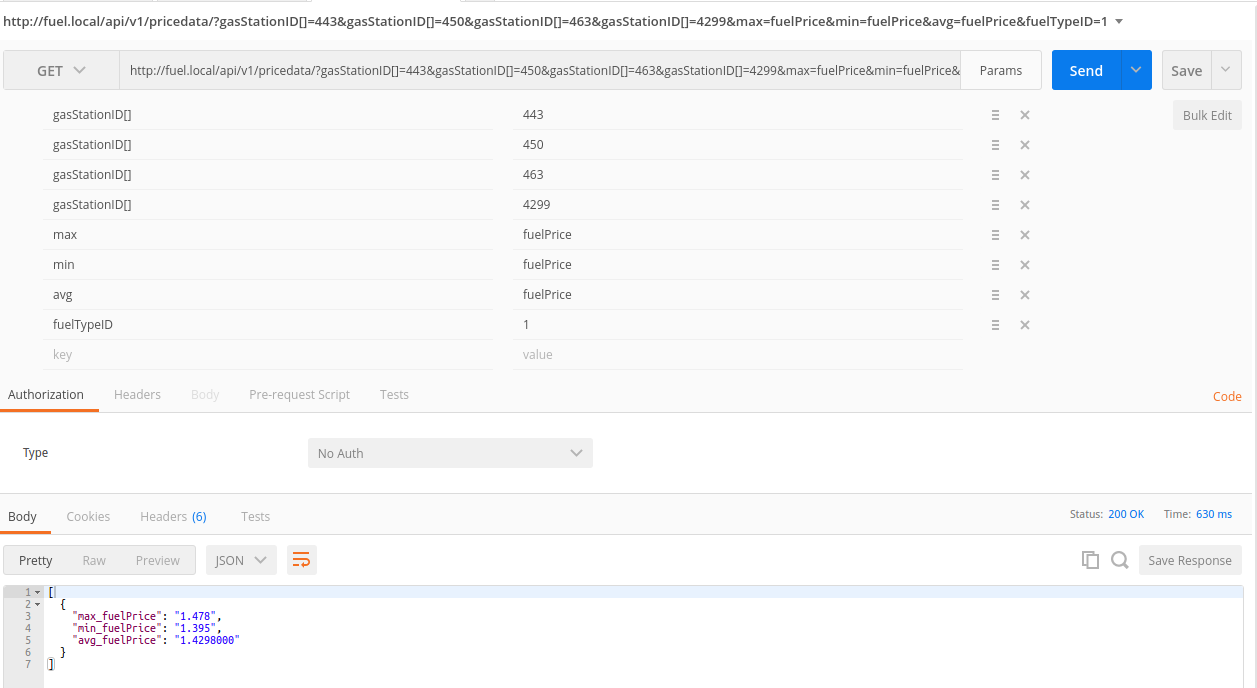
\includegraphics[width=1\textwidth]{img/max-min-postman.png}
    \label{fig:max-min-postman}
\end{figure}

\subsection{Λήψη τιμοκαταλόγου πρατηρίου}

\begin{figure}[H]
  \caption{Εικόνα πριν από τη λήψη τιμοκαταλόγου πρατηρίου.}
  \centering
    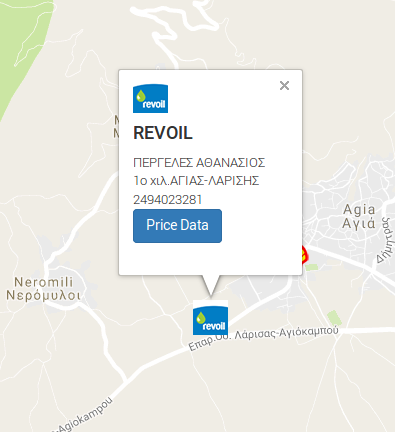
\includegraphics[width=1\textwidth]{img/pricedata1.png}
    \label{fig:pricedata1}
\end{figure}

\begin{figure}[H]
  \caption{Εικόνα μετά από τη λήψη τιμοκαταλόγου πρατηρίου.}
  \centering
    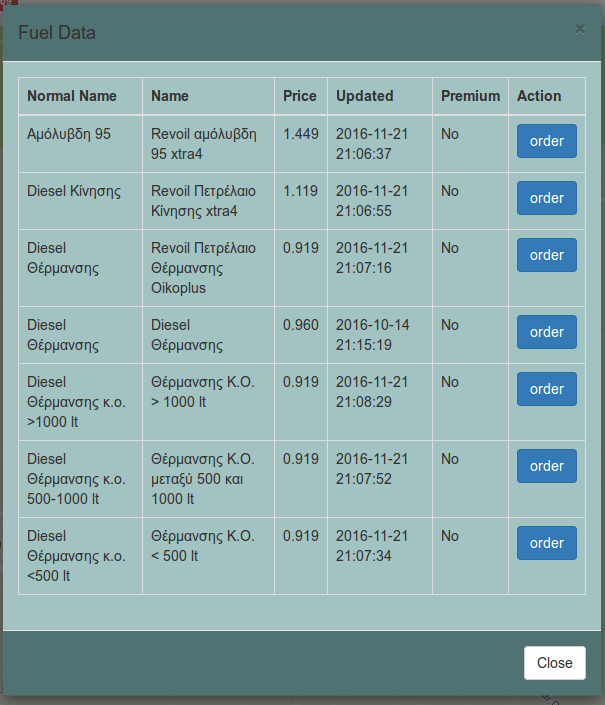
\includegraphics[width=1\textwidth]{img/pricedata2.png}
    \label{fig:pricedata2}
\end{figure}

\begin{figure}[H]
  \caption{Εικόνα με τη λήψη τιμοκαταλόγου πρατηρίου  από το request.}
  \centering
    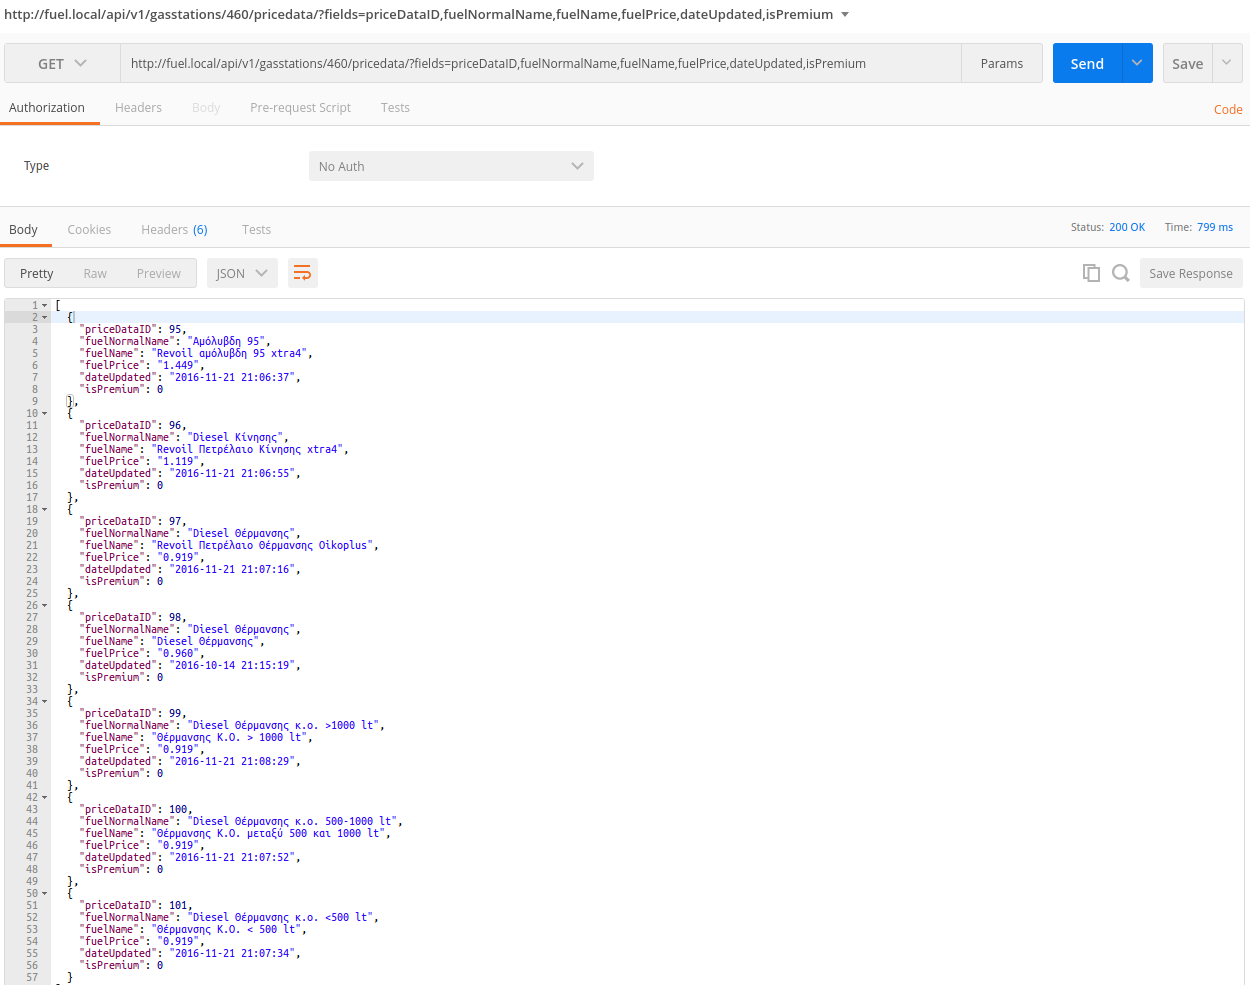
\includegraphics[width=1\textwidth]{img/pricedata3.png}
    \label{fig:pricedata3}
\end{figure}

\subsection{Λήψη δεδομένων πρατηρίων}

\begin{figure}[H]
  \caption{Εικόνα με τη λήψη δεδομένων πρατηρίων από το request.}
  \centering
    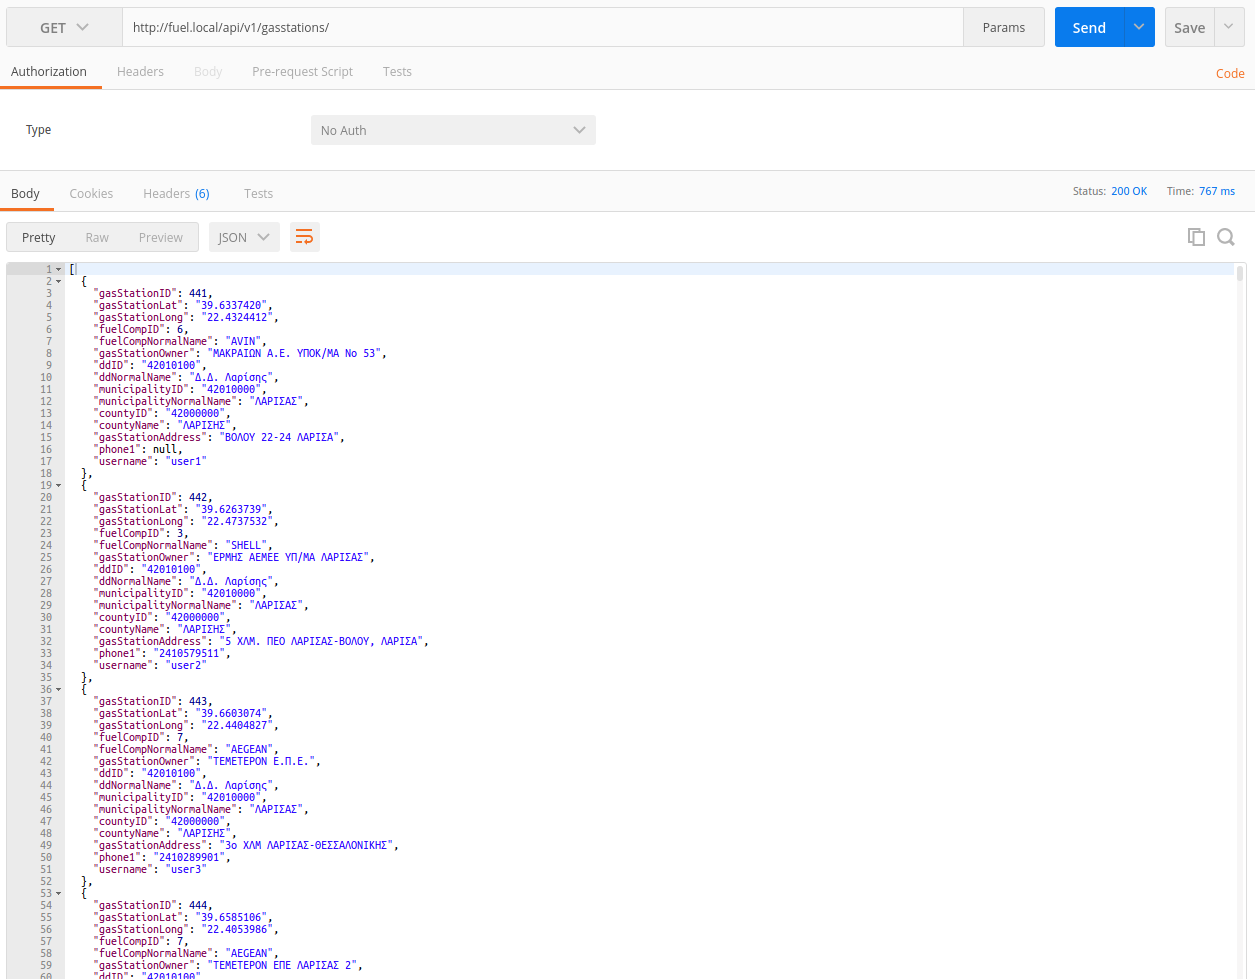
\includegraphics[width=1\textwidth]{img/gasstations.png}
    \label{fig:gasstations}
\end{figure}

\subsection{Έλεγχος παραγγελιών από πρατηριούχο}

\begin{figure}[H]
  \caption{Εικόνα με πριν τον ελεγχο παραγγελιών από πρατηριούχο.}
  \centering
    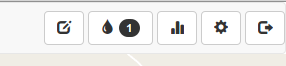
\includegraphics[width=1\textwidth]{img/pre-orders.png}
    \label{fig:pre-orders}
\end{figure}

\begin{figure}[H]
  \caption{Εικόνα κατά τον ελεγχο παραγγελιών από πρατηριούχο.}
  \centering
    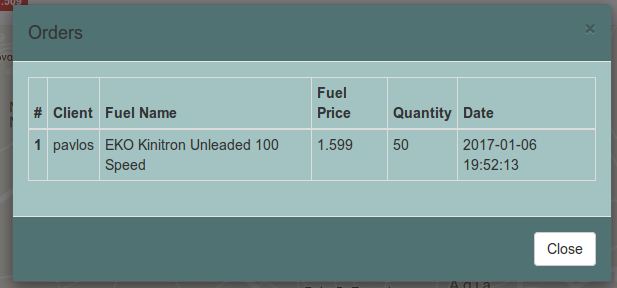
\includegraphics[width=1\textwidth]{img/orders.png}
    \label{fig:orders}
\end{figure}

\subsection{Ενημέρωση τιμών στο σύστημα από πρατηριούχους}

\begin{figure}[H]
  \caption{Εικόνα πριν την ενημέρωση τιμών.}
  \centering
    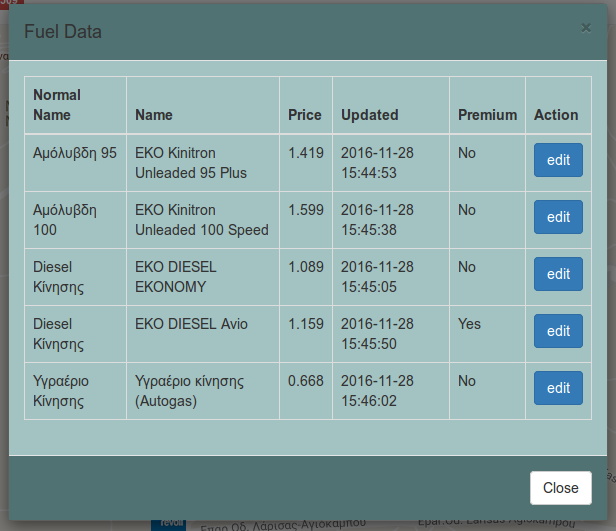
\includegraphics[width=1\textwidth]{img/pre-edit.png}
    \label{fig:pre-edit}
\end{figure}

\begin{figure}[H]
  \caption{Εικόνα κατά την ενημέρωση τιμών.}
  \centering
    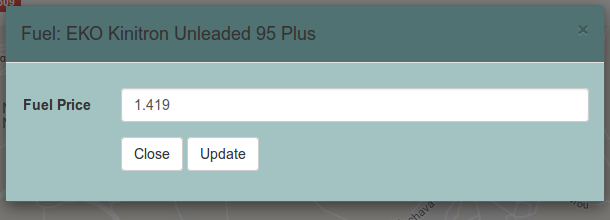
\includegraphics[width=1\textwidth]{img/pre-edit2.png}
    \label{fig:pre-edit2}
\end{figure}

\begin{figure}[H]
  \caption{Εικόνα μηνύματος μετά από την ενημέρωση τιμών.}
  \centering
    
\includegraphics[width=1\textwidth]{img/msg-edit.png}
    \label{fig:msg-edit}
\end{figure}

\begin{figure}[H]
  \caption{Εικόνα μετά από την ενημέρωση τιμών.}
  \centering
    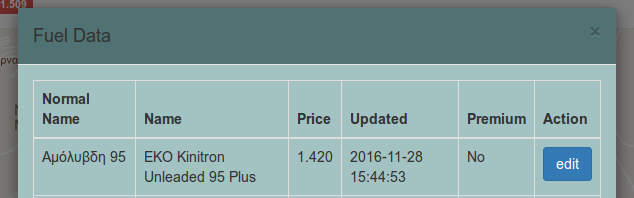
\includegraphics[width=1\textwidth]{img/after-edit.png}
    \label{fig:after-edit}
\end{figure}

\subsection{Αποστολή δεδομένων παραγγελίας από πλευράς χρήστη}

Εικόνα πριν την Αποστολή παραγγελίας. \ref{fig:pricedata1}

\begin{figure}[H]
  \caption{Εικόνα Login error κατά την Αποστολή παραγγελίας.}
  \centering
    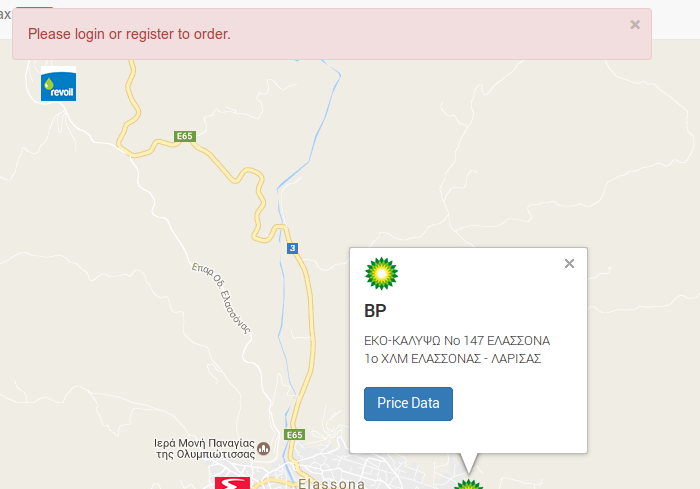
\includegraphics[width=1\textwidth]{img/make-order-error.png}
    \label{fig:make-order-error}
\end{figure}

\begin{figure}[H]
  \caption{Εικόνα quantity error κατά την Αποστολή παραγγελίας.}
  \centering
    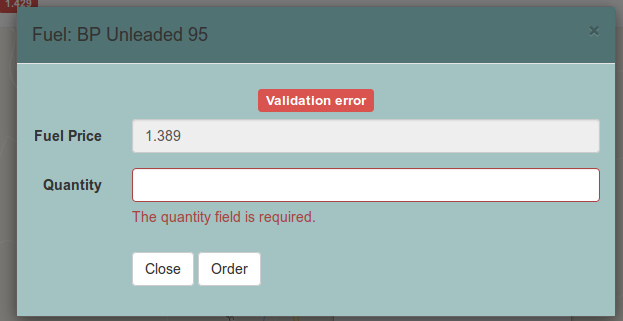
\includegraphics[width=1\textwidth]{img/make-order-error2.png}
    \label{fig:make-order-error2}
\end{figure}

\subsection{Επιλογή default fuel type για την απεικόνιση των max, min, avg τιμών}

\begin{figure}[H]
  \caption{Εικόνα επιλογής default fuel type.}
  \centering
    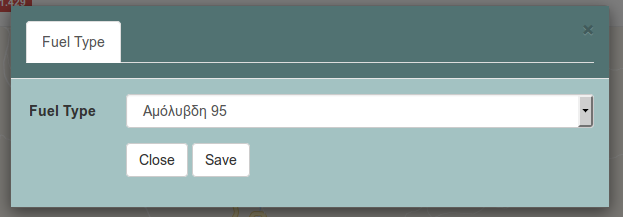
\includegraphics[width=1\textwidth]{img/fuel-type.png}
    \label{fig:fuel-type}
\end{figure}

\subsection{Μεταβίβαση σε επιλεγμένη περιοχή}

\begin{figure}[H]
  \caption{Εικόνα λάθους μεταβίβαση σε επιλεγμένη περιοχή.}
  \centering
    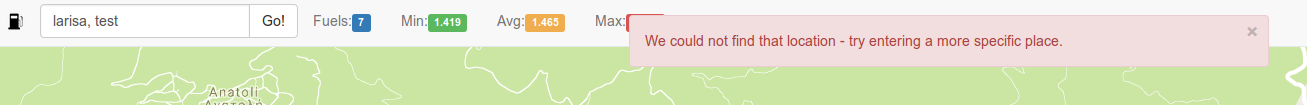
\includegraphics[width=1\textwidth]{img/area-error.png}
    \label{fig:arrea-error}
\end{figure}

\begin{figure}[H]
  \caption{Εικόνα πριν την μεταβίβαση σε επιλεγμένη περιοχή.}
  \centering
    
\includegraphics[width=1\textwidth]{img/pre-area.png}
    \label{fig:pre-area}
\end{figure}

\begin{figure}[H]
  \caption{Εικόνα κατά την μεταβίβαση σε επιλεγμένη περιοχή.}
  \centering
    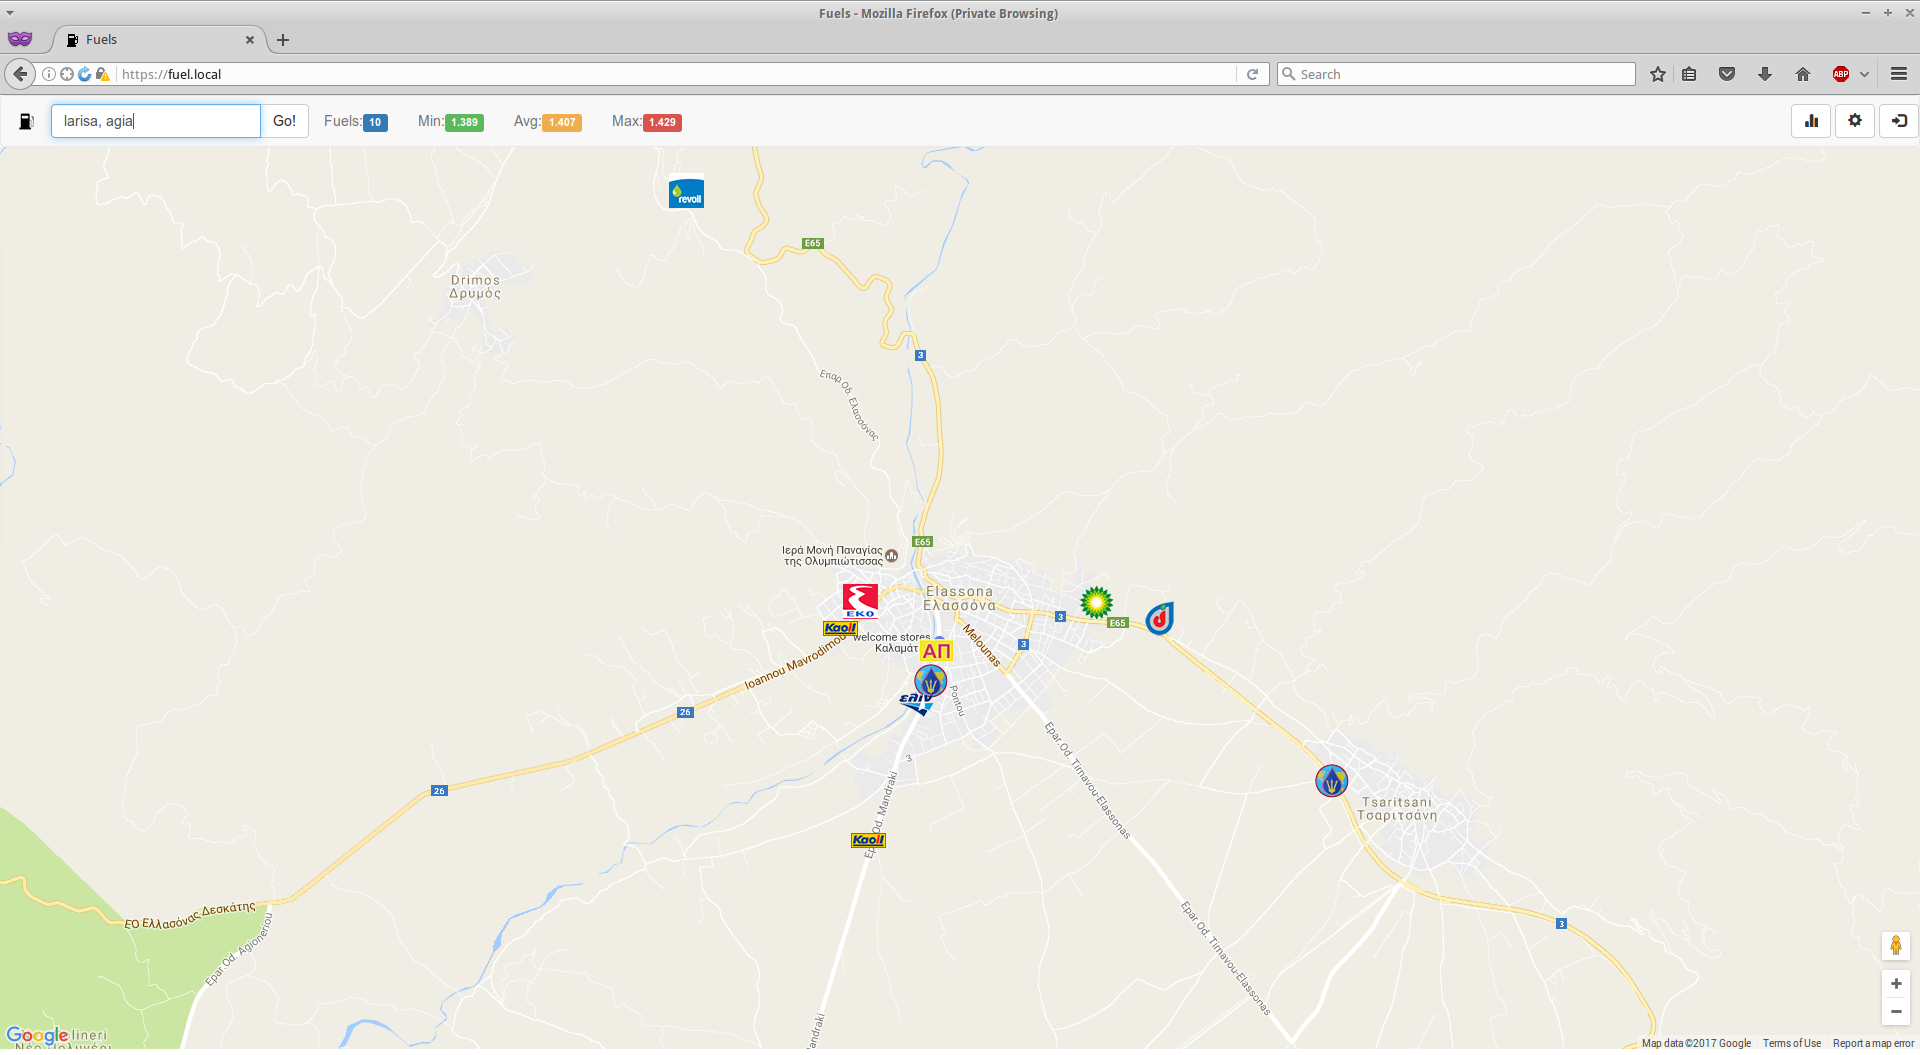
\includegraphics[width=1\textwidth]{img/area.png}
    \label{fig:area}
\end{figure}

\begin{figure}[H]
  \caption{Εικόνα μετά την μεταβίβαση σε επιλεγμένη περιοχή.}
  \centering
    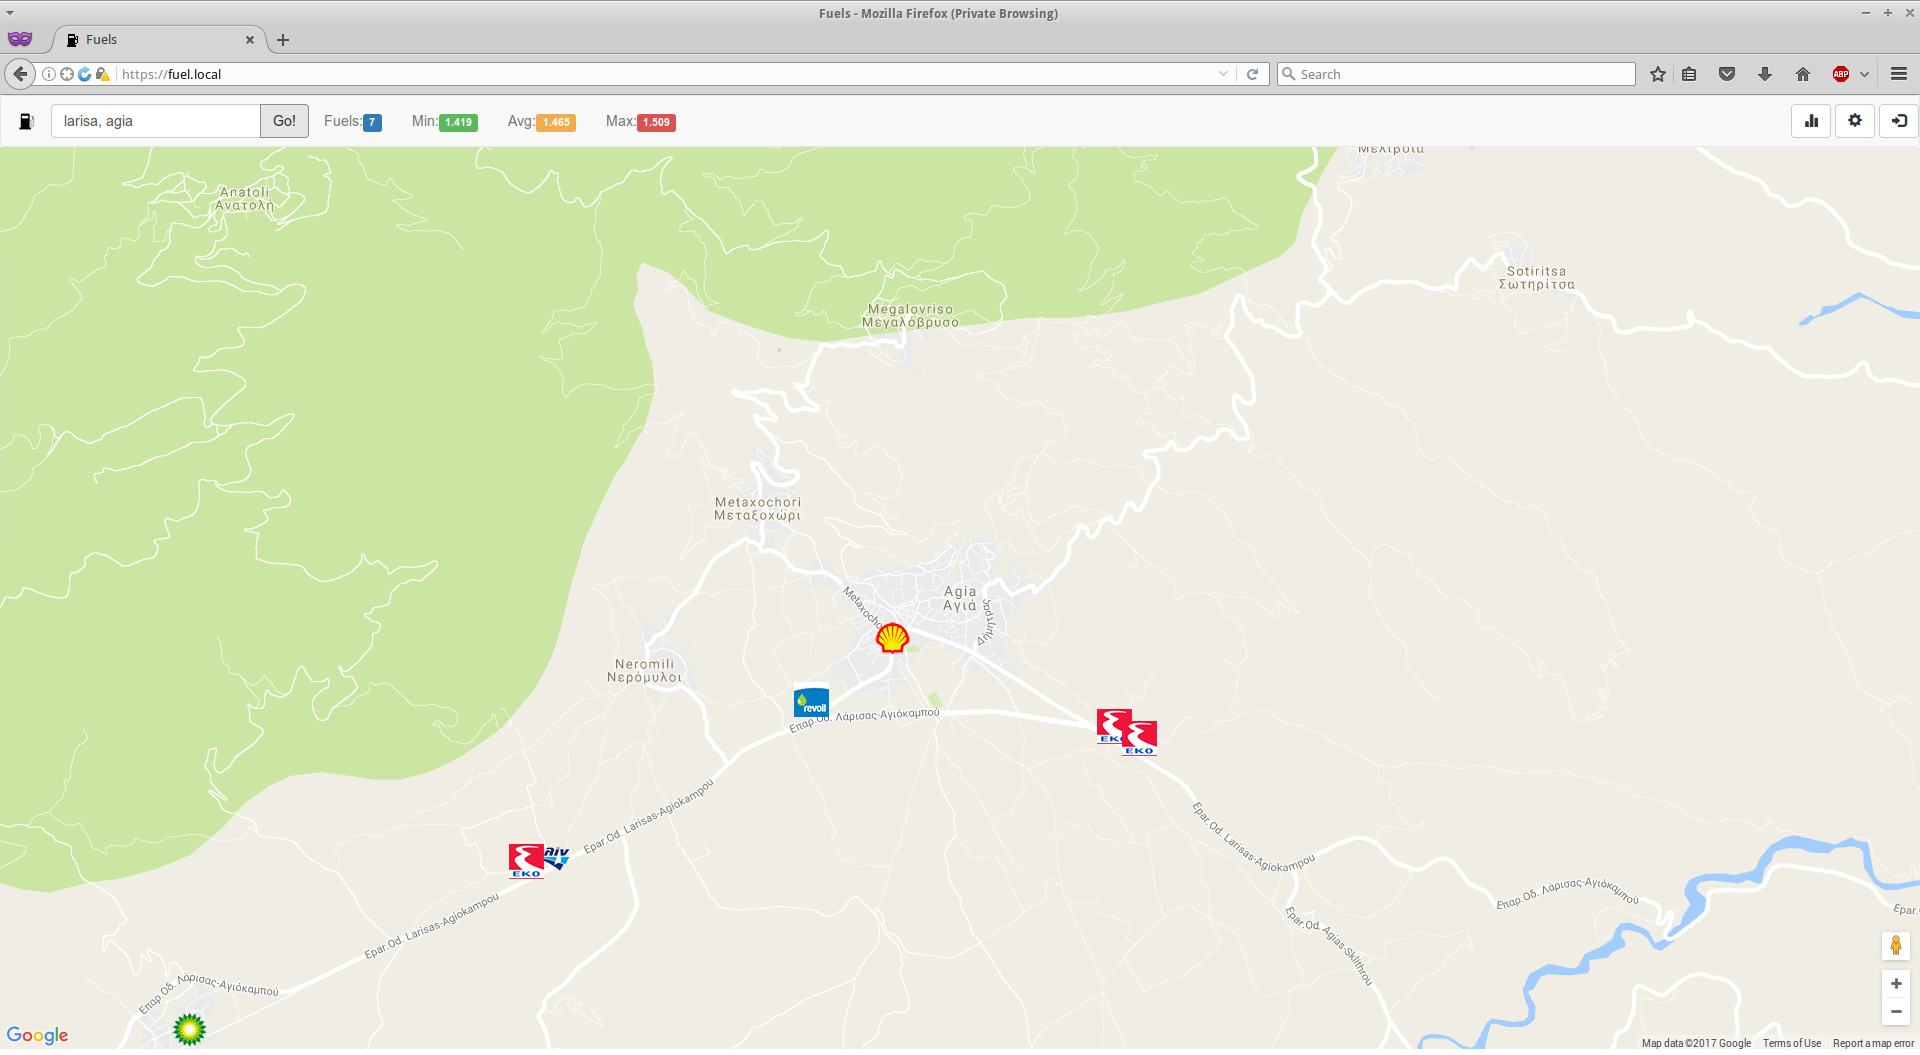
\includegraphics[width=1\textwidth]{img/area-after.png}
    \label{fig:area-after}
\end{figure}

\subsection{Επιλογή Geolocation}

\begin{figure}[H]
  \caption{Εικόνα κατά την Επιλογή Geolocation.}
  \centering
    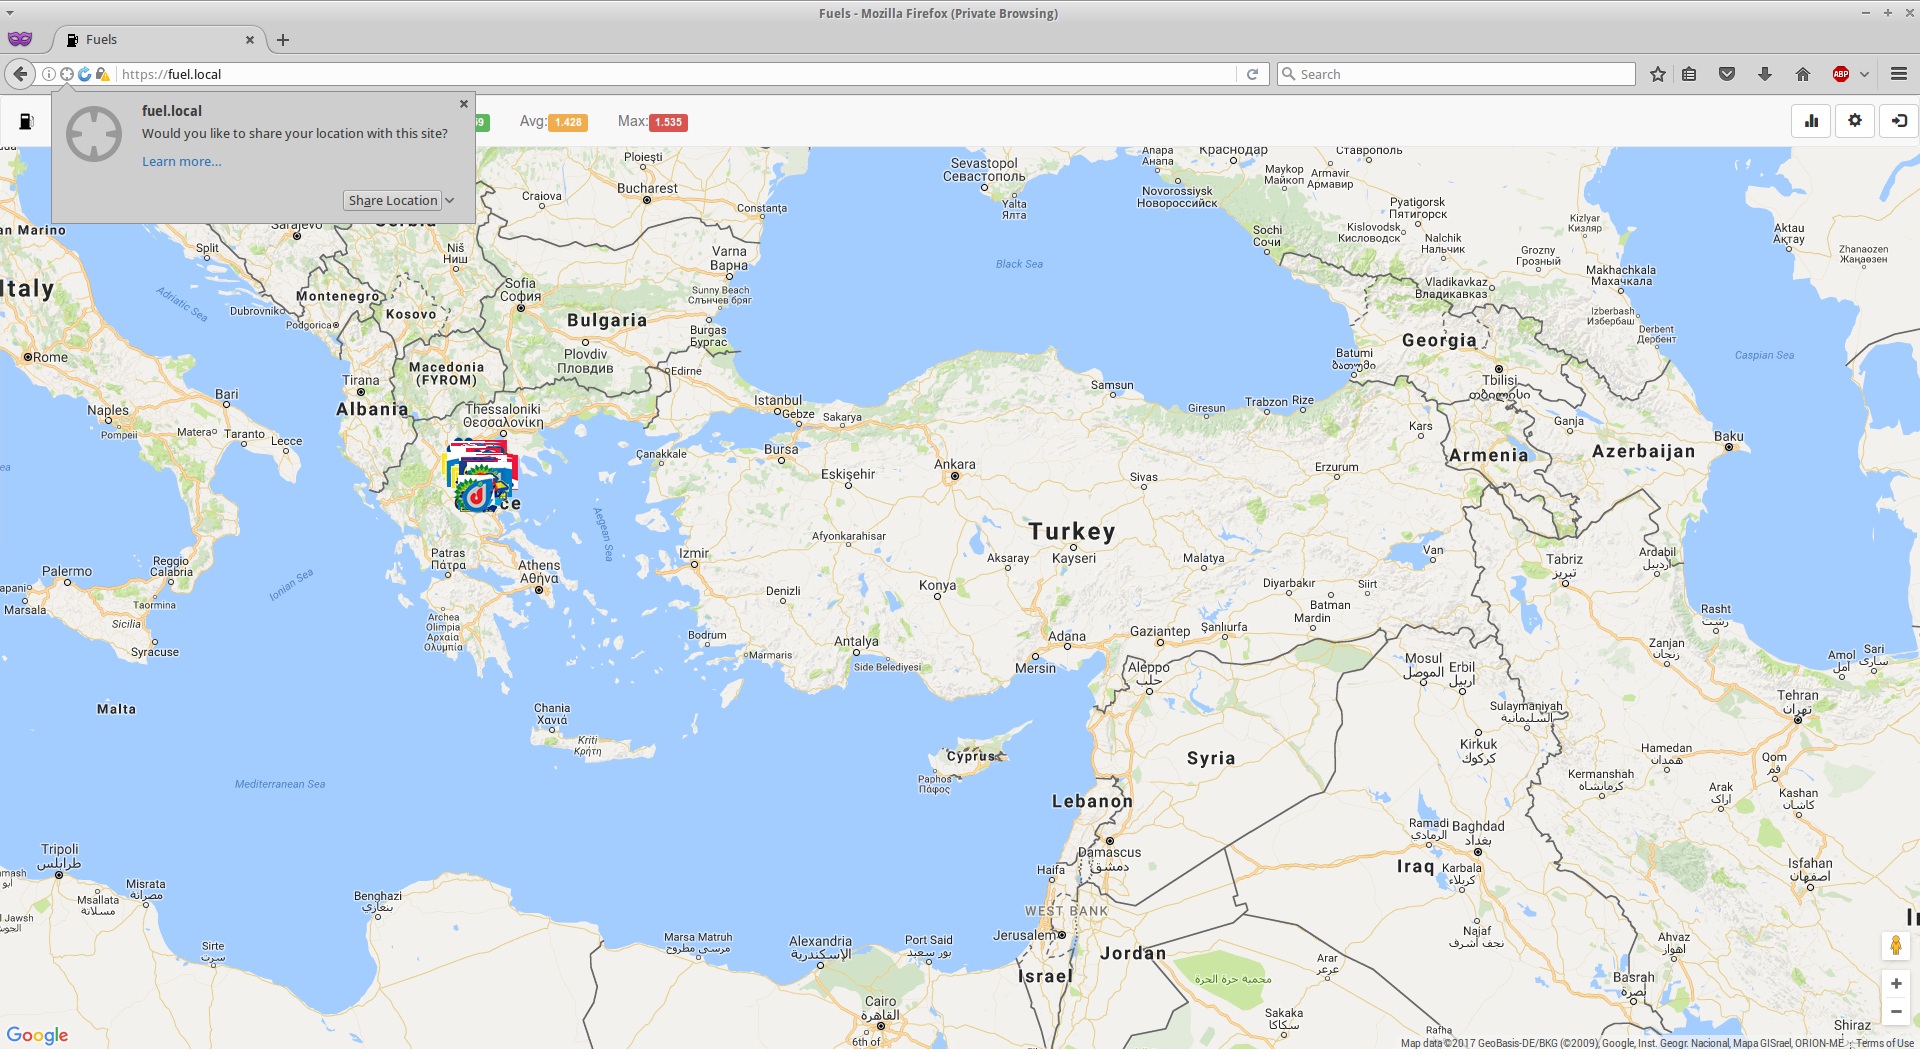
\includegraphics[width=1\textwidth]{img/geolocation.png}
    \label{fig:geolocation}
\end{figure}

Τα μηνύματα των φορμών καθώς και τα notifications προέρχονται κυρίως από το REST API.
	
%	\newpage
	
%	\input{sibe}
	
	\newpage
	
	\addcontentsline{toc}{section}{References}
	\bibliographystyle{plain}
	\bibliography{Report} 
\end{document}